\section{Background information}
\label{background}

The information in this sub section is not required for operating 
dvdisaster. However it is helpful for understanding how dvdisaster works 
and may help you getting the most out of the program according to your needs. 

\subsection{Properties of the error correction}
\label{background-properties}

This sub section outlines the basic ideas behind dvdisaster so that you can 
see for yourself whether it meets your demands on data safety. If in doubt, 
you should not use dvdisaster as a single means of protecting your data
and deploy additional data backup strategies.

\paragraph{Method of error correction.}   dvdisaster 
uses a \href{http://en.wikipedia.org/wiki/Reed-Solomon_error_correction}{Reed-Solomon code } together 
with an error correction algorithm optimized for the treatment of erasures. The 
implementation draws a lot of inspiration and program code from the 
excellent \href{http://www.ka9q.net/code/fec/}{Reed-Solomon} library written 
\href{http://www.ka9q.net/}{by Phil Karn}.

Using the \tlnk{howto-eccfile-basic-settings-ecc}{standard settings} of 
an \tlnk{howto-eccfile}{error correction} file 223 medium sectors 
are combined into one error correction code (``ECC'') block. 
Medium read errors are regarded as ``erasures''; therefore a maximum 
of 32 bad medium sectors\footnote{The given threshold of 32 correctable errors per ECC 
block is the standard setting. It is possible to select \tlnk{howto-eccfile-basic-settings-ecc}{other values} 
for higher or lower error correction capabilities. 
When \tlnk{howto-augment}{error correction data is put directly on the medium}, 
the number of correctable errors depends on the free space on the medium.} are 
correctable per ECC block.

The 223 sectors are selected so that they are evenly distributed over the medium 
surface. Therefore large contigous areas of defective sectors can be corrected before 
the threshold of 32 defects per ECC block is reached. This kind of error 
pattern is especially common for an aging medium where the outer area is starting 
to degenerate, and for scratches along the data spiral.

On the other hand, radial or diagonal scratches are expected to be correctable 
in the optical disc drive itself. If not, the employed error correction 
strategy performs rather neutral in these cases (neither especially good 
nor extraordinary bad).

\paragraph{Limits of error correction.} In the wost case, 33 defective sectors (for the
standard setting) are sufficient to prevent a full data restoration. However 
to achieve this effect, the errors have to be distributed over the medium in such 
a way that they occur in the same ECC block - such patterns are very unlikely.
Empirical tests have shown that on aging media about 10\% of the overall 
sector count may become defective before the threshold of 33 defects per ECC block is reached.
Scratches will cause the threshold to be reached earlier, therefore it is 
recommended to visually check the media in regular intervals. Media with read errors 
caused by scratches should be replaced immediately.

\paragraph{Hardware limits.}  Most drives will not recognize media when the 
lead-in area before the first sector (near the center hole) is damaged. 
In such cases, dvdisaster will not be able to recover any content from the media.

It is not feasible to enhance the reliability of poor quality media by using 
dvdisaster. Cheap media can decay within a few days to an extent which will 
exceed the capabilities of the error correction code. 

\subsection{Image level data recovery}
\label{background-image-level}

Media recovery with error correcting codes takes place in two steps:

\begin{enumerate}
\item First as much data as possible is read from the defective medium.
\item Then the still missing data is recovered using the error correction code.
\end{enumerate}

The amount of readable data (step 1) does not only depend on the reading 
capabilities of the drive, but also on which logical level the reading process 
takes place. This page discusses the logical levels and explains why dvdisaster 
uses image level reading. Please see also \tlnk{qa-image-level}{Q1.5} for
a visualization of this concept.

\paragraph{Logical levels of a medium.} Optical discs are organized into 
{\em data sectors} containing 2048 bytes each. Consecutively reading and storing 
these sectors produces a medium {\em image}.

But working with single data sectors is unwieldy from a users perspective. Therefore 
media contain {\em file systems} which combine data sectors into {\em files}. 
This requires accurate book-keeping about which data sectors each file is 
comprised of, and also further attributes like file names and access permissions. 
For this book-keeping some data sectors are reserved on the medium and filled 
with respective data structures.

As a consequence media contain different {\em logical levels}: Viewing the 
medium as a sequence of data sectors means working at the {\em image level}. 
However looking at the medium as a collection of files is the perspective of 
the {\em file(system) level}.

\smallskip

The two levels have different properties when it comes to data recovery:

\paragraph{Shortcomings of reading a medium at the file level.} Reading a defective 
medium at the file level means trying to read as much data as possible from each file.

But a problem arises when data sectors are damaged which have book-keeping 
functions in the file system. The list of files on the medium may be truncated. 
Or the mapping of data sectors to files is incomplete. Therefore files or parts 
from files may be lost even though the respective data sectors would still 
be readable by the hardware. This is very bad since even small readable portions 
of damaged files are valuable for the error correcting code.

An extremely bad case occurs when the error correction data is also stored in 
files. Then the error correction data is required to repair the file system, 
but the defective file system prevents access to the error correction data. 
That means total data loss and rises some issues on 
the treatment of error correction files (more on that later in this sub section).

A similar problem arises when files are augmented with PAR2 error correction 
data and then all these files are stored on the same medium. If the internal 
bookkeeping of the file system becomes damaged, all files and therefore the 
error correction data become inaccessible and are therefore lost.

\smallskip

However the situation improves greatly when employing an image-based approach:

\paragraph{Advantages of reading at the image level.} Reading at the image level 
uses direct communication with the drive firmware to access the data sectors.

The number of readable sectors depends only on the reading capabilities of the drive, 
but not on the state of the file system. A read error in one sector does not 
block access to other data sectors. Since {\em all} sectors are recovered 
which are still readable by the hardware, this method provides the best foundation 
for the error correction.

Another consideration is that the image contains all data sectors of 
the medium. When the image is completely 
recovered the file system stored within is also fully repaired. A protection 
at the image level is therefore more extensive than error correction at the file level.

dvdisaster is working exclusively at the image level to take advantage of these properties. 
The \tlnk{background-methods}{RS02 and RS03 methods} even allow 
for \tlnk{howto-augment}{storing the error correction data at the same medium}. 
This is possible since reading the error correction information at the image level 
can not be blocked by errors at other medium locations (damaged sectors with error 
correction data will reduce the error recovering capacity, but not make recovery impossible).

\smallskip

The \tlnk{background-methods}{RS01 method} protects media at the image level, too, 
but stores the error correction data in files. The next section hints at some pitfalls 
arising from that.

\paragraph{Consequences for error correction file storage.} \label{background-image-level-consequences}The error correction data 
created by dvdisaster protects media at the image level. But how are the error correction 
files protected?

\smallskip

Since error correction files are read at the file level they are subject to the 
problems discussed above. If the medium containing the error correction files 
becomes damaged it may not be possible to access or read them completely.

Therefore it is important to protect error correction files at the image level as 
well: \tlnk{background-eccfile-storage}{Media containing error correction files} must be 
protected with dvdisaster, too.

Since image level protection is assumed there is {\em no further damage protection}
contained in the RS01 error correction files! This would not help much, anyways: 
Error correction files could be created in a way that allows them to provide a 
reduced data recovering capacity even when being damaged\footnote{Error correction files 
created with the new RS03 codec have exactly these properties, e.g. they are robust 
against damage as long as there is enough error correction capacity left. This is 
possible as there is sufficient computing power and fast hard drive access available 
now to create a suitable file format. At the time RS01 was developed these resources 
were not yet available. But it must be stressed that even for RS03 error correction 
files the disadvantages of reading at the file level hold!}. But 
however such internal protection would be designed, the error correction file would 
still be only protected at the file system level with all the disadvantages discussed above!

In addition, the computing time and redundancy used for internal protection is 
better spent at the image level: The Reed-Solomon error correction works best
 when error correction information is spread over huge amounts of data. It is 
better to protect the image as a whole than individually protecting each file within.

 
\subsection{The RS01, RS02 and RS03 methods}
\label{background-methods}

dvdisaster contains three error correction methods.
RS01 and RS02 have been available right from the start of the project.
RS03 has been added recently to take advantage of 
recent hardware, and to implement improvements
learned from evaluating its predecessors.

\paragraph{Comparison of the methods.} All three methods build on the 
same \tlnk{background-properties}{Reed-Solomon} error correction. They calculate error 
correction information for ISO images which is used to recover unreadable sectors if 
the disc becomes damaged afterwards.

\smallskip

The methods differ in the way the error correction information is stored:

\begin{itemize}
\item  RS01 creates {\bf error correction files} which are stored separately 
from the image they belong to. Since data protection at 
the \tlnk{background-image-level}{file level} is difficult, 
error correction files must be stored on media which are protected against data loss by dvdisaster, too.

\item To apply the RS02 method an image is first created on hard disk using a 
optical disc authoring (or writing) software. Before the image is written on the medium, 
dvdisaster is used to {\bf augment the image} with error correction data. 
Therefore the data to be protected and the error correction information are located at 
the same medium. Damaged sectors in the error correction information reduce the data recovering 
capacity, but do not make recovery impossible - a second medium for keeping or protecting the 
error correction information is not required.
\end{itemize}


RS03 is a further development of RS01 and RS02. 
It can create both error correction files and augmented images:

\begin{itemize}
\item RS03 can distribute work over multiple processor cores and is 
therefore much faster than RS01/RS02 on modern hardware.
\item RS03 {\bf error correction files} are - contrary to RS01 - robust 
against damage. This should not delude you into careless handling of your error 
correction files though - the disadvantages of \tlnk{background-image-level}{reading at the filesystem level} are 
still valid.
\item RS03 {\bf augmented images} do not require so-called master blocks 
holding important information. This makes RS03 a bit more robust, but also more restrictive: 
The augmented image must completely fill the medium now while the size of augmented images 
can be freely chosen in RS02.
\end{itemize}

The changes for parallel computation and higher robustness make RS03 a bit less space efficient, 
e.g. RS03 error correction data has slighly less error correction capacity than 
its RS01/RS02 counterparts on images with equal size.

\newpage

\paragraph{Comparison of error correction storage.} The following table summarizes the differences 
between error correction files (RS01, RS03) and augmented images (RS02, RS03):

\smallskip

\begin{tabular}{|p{0.473\textwidth}|p{0.473\textwidth}|}
\hline
{\em Error correction files} 	& 
{\em Image augmented with error correction data} \\
\hline
any possible redundancy can be chosen &	
redundancy is limited by free space on the medium (= medium capacity - size of data image) \\
\hline
already effective at 15\% redundancy since error correction files are required to be free of damage &
requires more redundancy (recommended: 20-30\%) to compensate defects in the error correction data \\
\hline
medium can be completely filled with data  &
usable medium capacity is reduced by amount of error correction data \\
\hline
can be created for already existing media & 
only applicable before writing the new medium since the image must be augmented with error correction information in advance \\
\hline
separately storing the error correction file from user data strengthens data protection &
common storage of user data and error correction data may reduce error correction capacity \\
\hline
mapping between error correction files and media must be kept; error correction files must be 
protected against damage &
easy one-medium solution; error correction information needs not to be cataloged or explicitly protected \\
\hline
no compatibility issues with play-back units &
media with augmented images may not play correctly on all units \\
\hline
\end{tabular}

\paragraph{Further reading.} The specification for the dvdisaster codecs 
has been specified in a separate document called \href{http://dvdisaster.net/downloads/codecs.pdf}{codecs.pdf}. 
Good knowledge in coding theory and programming is required.

\subsection{The linear reading strategy}
\label{background-linear}

dvdisaster contains two different reading strategies.

\medskip

{\bf The linear reading strategy is recommended for:}

\begin{itemize}
\item Creating images from undamaged media,
  e.g. to \tlnk{howto-eccfile}{generate the error correction file}; and
\item \tlnk{howto-scan}{Scanning the medium} for reading speed and read errors.
\end{itemize}

\medskip

{\bf The} \tlnk{background-adaptive}{adaptive reading strategy} {\bf is recommended for:}

\begin{itemize}
\item \tlnk{howto-recover}{Extracting data from damaged media.}
\end{itemize}

\paragraph{Properties of the linear reading strategy.}\quad

\medskip

Optical media are
organized into sectors which are continously numbered beginning with zero.
Each sector contains 2048 bytes of data.

\begin{figure}
\centerline{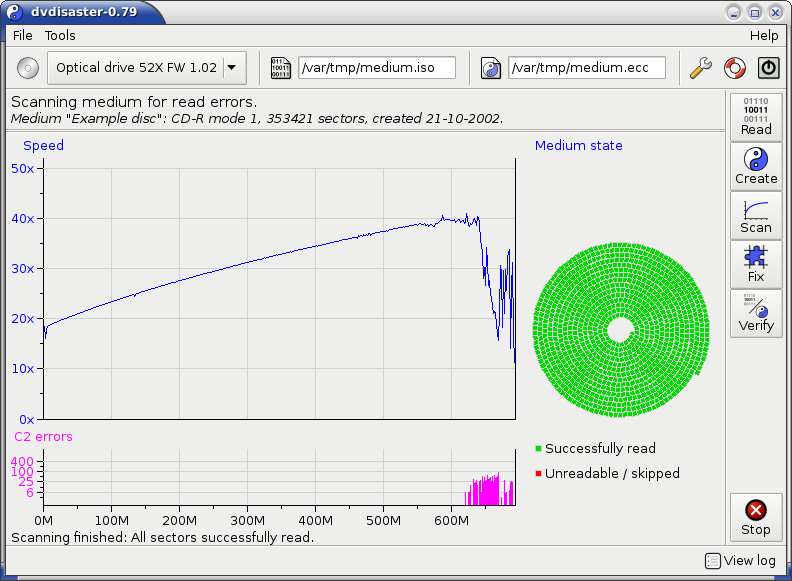
\includegraphics[width=1.0\textwidth]{screenshots/weak-cd-scan.png}}
\caption{Linear reading of a weak but fully readable CD.}  
\label{background-linear-weak-scan}
\end{figure}

The linear reading strategy reads the medium from the start (sector 0)
until the end (last sector). The reading speed is shown graphically to
provide information about the medium quality (see
figure \ref{background-linear-weak-scan} for an example and the explanations
in the following paragraphs). 

\paragraph{Configuration.}\quad

\medskip

\paragraph{Number of sectors to skip after a read error.} Reading
attempts for defective sectors are slow and may wear out the drive
mechanics under unfavourable conditions. A series of read errors,
spread over a continous sector range, is more common than single spot defects.
Therefore a \tlnk{howto-scan-prefs-read-attempts}{configuration option} exists
so that a certain number of sectors
will be skipped after the occurance of a read error. The skipped sectors are
assumed to be defective without further reading attempts. Some guide lines for
selecting the number of skipped sectors are:

\begin{itemize}
\item Skipping a large number of sectors (e.g. {\bf 1024}) gives a quick
  overview of the degree of damage, but will usually not collect enough
  data for repairing the medium image.
\item Smaller values like {\bf 16, 32 or 64} are a good trade-off: The processing
  time will be considerably shortened, but still enough data for repairing
  the image is usually collected.
\item On DVD and BD  media read errors do usually extend over at least 16 sectors
  for technical reasons. Therefore a sector skip less than 16 is not recommended
  for such  media.
\end{itemize}

\paragraph{Limiting the reading range.}

\medskip

Reading can
be \tlnk{howto-scan-prefs-image}{limited to a given range of sectors} in
the ``Image'' preferences tab. This is helpful during
multiple read attempts of damaged media. 

\paragraph{Estimating media quality.}\quad

\medskip

\paragraph{The speed curve.} Most drives
will slow down while reading medium areas which are in bad condition:

\begin{itemize}
\item Drops in the reading speed can be a warning for an imminent medium failure.
\item However some drives will read with full speed until the bitter end.
  With such drives media deterioration may not show up in the reading
  curve until actual read errors occur.
\end{itemize}

  The reading curve is most accurate when using
  the ``\tlnk{howto-scan}{Scan}'' function.
  During the ``\tlnk{howto-eccfile-create}{Read}'' operation the
  read data will be written to the hard
  drive at the same time, which may cause irregularities in the reading curve
  depending on the operating system and hardware used.

\paragraph{Read errors.} Read errors cause \tlnk{howto-interpret-defective-cd}{red markings} in
the spiral or respective messages at the command line. This means
that the medium could not be read at these places during the current reading pass:

\begin{itemize}
\item The medium is most likely defective.
\item The image should be \tlnk{howto-recover}{repaired} as
  soon as possible and then be transferred to a new medium.
\end{itemize}

\subsection{The adaptive reading strategy}
\label{background-adaptive}

Please note: Adaptive reading is unavailable in the current
version of dvdisaster as it requires rework for RS03. It
will be re-introuced soon. It is documented here for completeness:
%dvdisaster contains two different reading strategies.

\medskip

{\bf The adaptive reading strategy is recommended for:}

\begin{itemize}
\item \tlnk{howto-recover-read}{Extracting data} from damaged media,
\end{itemize}

\medskip

{\bf The} \tlnk{background-linear}{linear reading strategy} {\bf is recommended for:}

\begin{itemize}
\item \tlnk{howto-eccfile-create}{Creating images} from undamaged media,
  e.g. to generate the error correction file.
\item \tlnk{howto-scan}{Scanning the medium} for reading speed and read errors.
\end{itemize}

\paragraph{Properties of the adaptive reading strategy.}\quad
\medskip

The adaptive reading strategy uses a ``divide and conquer'' approach for locating still readable portions of a damaged medium. The strategy is based upon an article published by Harald Bögeholz in c't-Magazin 16/2005 where it was published together with the program {\em h2cdimage}:

\begin{enumerate}
\item At the beginning the medium is considered as a single unread interval.
  Reading begins with sector zero.
\item The reading process continues sequentially unless either the end of the
  current interval or a read error is encountered.
\item The reading process is terminated if either (3a) sufficient sectors for
  a successful error correction have been read or (3b) no unreadable intervals
  exceeding a given size remain.
\item Otherwise the largest remaining unread interval will be determined. Reading
  continues in the middle (e.g. second half) of this interval; the first half of
  this interval is kept for a later reading pass.
\end{enumerate}

\begin{figure}
\centerline{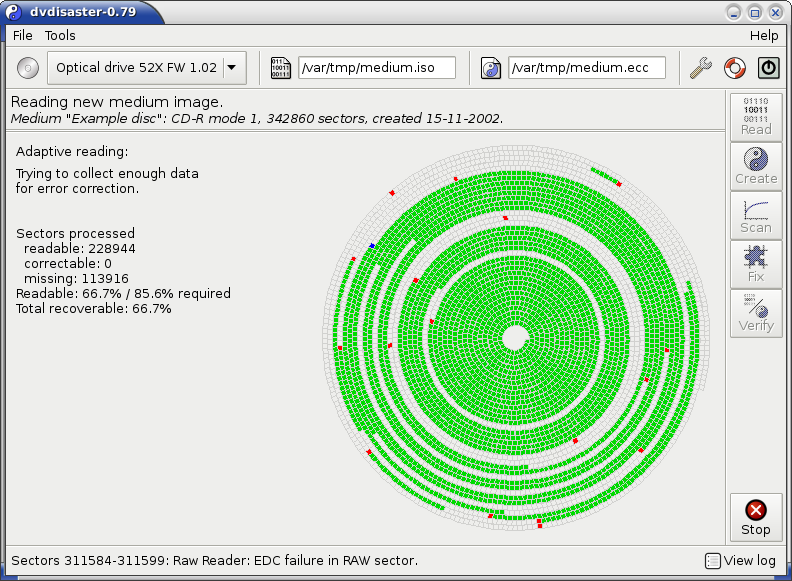
\includegraphics[width=1.0\textwidth]{screenshots/adaptive-progress.png}}
\caption{Progress of th adaptive reading.}  
\label{background-adaptive-progress}
\end{figure}

The termination criterium (3a) is especially efficient: Reading
will stop as soon as enough sectors have been collected for a
successful image recovery using the error correction file. This
can reduce the reading time by as much as 90 percent compared
with a full read attempt, but does of course only work when
error correction data is available.

\paragraph{Configuration}\quad

\medskip

\paragraph{Error correction file.} Adaptive reading works best when error
correction data is available. Obviously the \tlnk{howto-ecc}{error correction data} must have
been created at a time where the medium was
still fully readable. To use a \tlnk{howto-eccfile-create}{error correction file} during 
adaptive reading,
\tlnk{howto-recover-enter-eccfile}{enter its name} before starting the reading process.

\paragraph{Limiting the adaptive reading range.} Reading can
be \tlnk{howto-eccfile-prefs-image}{limited} using the ``Image'' preferences
to a part of the medium. This is not recommended
when error correction data is used since the limit might prevent sectors
from being read which are required for a succesful error correction. If
no error correction data is available, limiting the reading range might
be helpful during multiple reading attempts.

\paragraph{Early reading termination.} If no error correction
data is available, adaptive reading will stop when no unread intervals
\tlnk{howto-recover-prefs-read-attempts}{larger than a selectable size} remain.

The termination value should not be smaller than 128. Otherwise the laser
head will have to carry out lots of repositioning moves during the final
phase of the reading process. This will negatively affect both the life
expectancy of the drive and its reading capability. A better approach is
to stop adaptive reading earlier and then try reading the remaining sectors
with an additional \tlnk{background-linear}{linear reading} pass. 

\subsection{Remarks on read errors}
\label{background-read-errors}

Optical media have their own error correction code which protects the data against
small manufacturing errors and inaccuracies during writing. If the writer and medium
are compatible and of high quality, the error correction built into the medium will
at first be mainly idle. This leaves enough reserves to compensate normal wear and
aging effects during many years of the medium usage.

\smallskip

When the capacity of the built-in error correction is finally exhausted, read errors
will start to appear on the medium. These will be reported by
the ``\tlnk{howto-scan}{Scan}''-operation
of dvdisaster. Depending on the time of first occurrence, two types of read errors
are of particular interest:

\paragraph{Read errors appearing right after writing the medium.} This is a sign of:

\begin{itemize}
\item media from a faulty production run, or
\item media which are not compatible with the writer.
\end{itemize}

A prudential choice is to dispose of the faulty media and to write the data
on error-free media, possibly switching to a different producer.

\smallskip

Please withstand the temptation of trying to preserve the faulty media
by means of an error correction file - this will most likely end with data loss.

\paragraph{Read errors after a few months/years.} The built-in error correction
of the medium will be increasingly loaded during its life time until it finally
fails and read errors show up. This happens for mechanical reasons (scratches,
warping of the plastic material) as well as for chemical causes (decaying dye
and/or reflective layer).

\smallskip

These effects typically occur while the medium is stored away for a few months,
and it may not be possible to read in all sectors afterwards.

\smallskip

Therefore it is crucial to \tlnk{howto-ecc}{create the error correction data} in
time. The ecc data contains information for recalculating the contents of missing
sectors (\tlnk{background-properties}{within certain limits}).
Therefore with the help of the ecc data dvdisaster can recover images even
if not all sectors could actually be read by the drive.

\smallskip

Since the error correction can reconstruct missing sectors up to a certain number,
it is not necessary to squeeze out a defective medium for every readable sector.
The \tlnk{background-adaptive}{adaptive reading strategy} checks during reading
whether enough data for error correction has been collected. As soon as this is
the case, reading stops and still unread sectors will be recovered using the ecc data.

\paragraph{Some hints for effectively reading damaged media}\quad

\medskip

The outcome from reading damaged media depends on several factors:

\begin{itemize}
\item {\bf Not all drives are built the same.}
  
  Different drives have different reading capabilities. Take advantage of dvdisaster's
  function for completing an image with several reading passes and use different drives
  for each pass. Transfer the image file between computers using a network or removable
  media in order to use drives installed in different machines.

\item {\bf Eject and insert the medium again.}
  
  Sometimes it makes a difference to eject the medium, turn it about a quarter,
  and then load it again for another reading pass.

  \item {\bf Some drives read better while being cold.}

    Turn off the computer over night and perform another reading attempt in the next morning.

    But note: ``Cold'' refers to normal living room conditions - putting hardware or
    media into the fridge can be very unhealthy for them.
 \end{itemize}


\subsection{Hints for storing the error correction files}
\label{background-eccfile-storage}

Currently there are few (if any) exchangeable media technologies which can be a
cost-effective alternative to the various optical disc formats. So you will
probably not only use optical discs for data archival, but store the respective
error correction files on CD, DVD or BD as well.

\smallskip

There is nothing wrong with that, but bear in mind that your archived data and
the error correction files are stored on media with the same degree of reliability.
When read errors occur on the archived data, be prepared that the disc with the
respective error correction file might have aged beyond full readability, too.

\smallskip

Therefore it is important to protect your error correction files with the same
care as your other data\footnote{You might also choose
  an \tlnk{howto-augment}{augmented image} using RS02 or RS03 instead
  of creating an error correction file.}.
This is best achieved by integrating the error correction files into
your normal data backup scheme. Here are two ideas:

\paragraph{1. Storing the error correction files on dedicated media:}\quad
\medskip

If you decide to store error correction files on separate media, it
is \tlnk{background-image-level-consequences}{important} to protect those media
with dvdisaster as well. To avoid a never-ending chain (error correction
files for media of error correction files for ...), try the following:

\smallskip

Lets assume that five error correction files can be stored at each medium.
Write the first five error correction files to the first medium and create
another error correction file for that medium. Now save that error correction
file together with four other error correction files on the second medium.
If you continue that way, all error correction files except for those from the
last medium (which may still be kept on hard disk) are protected by dvdisaster.

\paragraph{2. Putting the error correction file on the next medium of a series:}\quad
\medskip

If you do not fill your media to the max (e.g. with less than 4GiB for
a single layered DVD), you can store the error correction file of one
medium on the succeeding medium within a series.

 
